\documentclass{article}
\title{Ongoing Thesis Writeup}
\author{Michael Buch}
\date{\today}

\usepackage[inline]{enumitem} % inline numbered lists
\usepackage[left=2cm,right=2cm]{geometry}
\usepackage{verbatim} % for comments
\usepackage{graphicx}
\usepackage{hyperref}
\hypersetup{
    colorlinks=true,
    linkcolor=blue,
    filecolor=magenta,      
    urlcolor=cyan,
}
\urlstyle{same}

\begin{document}
\maketitle
\frenchspacing

\newcommand{\mslang}{$\lambda\uparrow\downarrow$}
\newcommand{\mslangStar}{$\lambda\uparrow\downarrow^*$}

\section{About this document}
This is a collection of references and summaries to research in the field of meta-programming/supercompilation/partial evaluation

\section{An Introduction to Towers of Interpreters}
\subsection{LISP-3, Metacircularity and Reflection}
In his proposal for a language extension to Lisp called LISP-3 \cite{smith1984reflection}, Smith introduces the notion of a reflective system, a system that is able to reason about itself. He argues that reflection is not a property that metacircular interpreters languages provide, but additionally requires a way with which an embedded language can access structures of the system it was described in in its own terms. LISP-3 achieves this by way of a, conceptually infinite, reflective tower. Crucial is the idea of implicit as opposed to explicit information about a system during computation. Smith's idea of reflection is the ability to explicitly instantiate a language construct that was implicit prior. While environment and continuations, which form the state of the Lisp process, are implicitly passed around, a LISP-3 program can access both these structures explicitly at any point in time.
\subsection{A Formal Account}
Friedman et al. took Smith's account of reflection and decomposed it into processes called reification and reflection \cite{friedman1984reification}.
\cite{wand1988mystery}
\cite{danvy1988intensions}: starts with a non-reflective tower (and not strictly meta-circular) WHICH IS EXACTLY WHAT WE WANT and turns it into a reflective tower

\subsection{Tower Semantics}
\subsection{Compiling Reflective Languages}
\cite{asai1996duplication}: Language ``Black''; has early uses of the act of collapsing modes of interpretation in a reflective setting. Its reflective model is closer to 3-LISP than to Blond or Brown
\cite{asai2015compiling}
\subsection{Heterogeneity}
So far we have only discussed towers that were homogeneous in nature. We define homogeneous as the combination of metacircularity and reflectivity of interpreter embeddings. A consequence of homogeneity are small semantic gaps throughout levels.
\cite{sturdy1993lisp}
First part of \cite{danvy1988intensions}

\subsection{Coming Full Circle: Partial Evaluation, Reflective Towers (and Supercompilation)}

\section{Examples}
Examples drawn from paper on collapsing towers \cite{amin2017collapsing}:
\begin{itemize}
	\item Regular expression matcher <- Evaluator <- Virtual Machine
	\begin{itemize}
		\item Generate low-level VM code for a matcher specialized to one regex (through arbitrary number of intermediate interpreters)
	\end{itemize}
	\item Modified evaluator <- Evaluator <- Virtual Machine
	\begin{itemize}
		\item Modified for tracing/counting calls/be in CPS
		\item Under modified semantics "interpreters become program transformers". E.g. CPS interpreter becomes CPS transformer
	\end{itemize}
\end{itemize}

\section{Methodologies Background}
\begin{itemize}
	\item Stage polymorphism \cite{ofenbeck2017staging}: ``abstract over staging decisions'' i.e. single program generator can produce code that is specialized in many different ways (instance of the Fourth Futamura Projection? \cite{gluck2009there}) 
	\item Multi-level base evaluator written in \mslang: supports staging operators (\textbf{polymorphic Lift})
	\item Modify other interpreters: make them \textbf{stage polymorphic}, i.e. commands either evaluate code (like an interpreter) or generate code (like a translator)
	\item Stage only user-most interpreter: \textit{wire tower} such that the \textbf{staging commands in $L_{n}$ are interpreted directly in terms of staging commands in $L_{0}$} i.e. staging commands pass through all other layers handing down commands to layers below without performing any staging commands
	\item Non-reflective method: meta-circular evaluator \textbf{Pink} => collapse arbitrary levels of ``self-interpretation''
	\item \mslang features:
	\begin{itemize}
		\item \textit{run residual code}
		\item binding-time/stage polymorphism \cite{henglein1994polymorphic}
		\item preserves execution order of future-stage expressions
		\item does not require type system or static analysis
		\begin{itemize}
			\item TDPE \cite{danvy1999type} (great explanation also at \cite{grobauer2001second}): \textbf{polymorphic Lift} operator turns static values into dynamic (future-stage) expressions
		\end{itemize}
	\end{itemize}
\end{itemize}

\subsection{Towers of Interpreters Project Overview}
\subsubsection{Scala}
\begin{itemize}
	\item base.scala: implements definitional interpreter for \mslang
\end{itemize}

\section{Results}
\begin{itemize}
	\item Able to achieve compilation of stack-machine on top the Pink evaluator (including tracing evaluator etc.)
	\item Compilation i.e. collapsing through explicit staging annotations requires intricate knowledge of infrastructure and does not support all data structures e.g. stacks
\end{itemize}

\subsection{Benchmarks}
We extended the benchmarks provided as part of the original framework \cite{amin2017collapsing} with timings for staging the stack machine with respect to a user factorial program and timings for evaluating said program.
The compilation output yielded and is essentially a loop unrolling of the (non-recursive SECD) factorial program without traces of the SECD emulator left:
\begin{verbatim}
	Let(
		Gt(Lit(3),Lit(1)),
		Let(
			Equ(Var(3),Lit(0)),
			Let(
				If(Var(4),
					Lit(1),
					Let(
						Lift(Sym(.)),
						Let(
							Cons(Lit(3),Sym(.)),
							Let(
								Fst(Var(6)),
								Let(
									Minus(Lit(1),Var(7)),
									Let(
										Times(Var(8),Lit(-1)),
										Let(
											Fst(Var(6)),
											Let(
												Times(Var(9),Var(10)),
												Let(
													Snd(Var(6)),
													Let(
														Minus(Lit(1),Var(7)),
														Let(
															Times(Var(13),Lit(-1)),
															Let(
																Minus(Lit(1),Var(14)),
																Let(
																	Times(Var(15),Lit(-1)),
																	Let(
																		Times(Var(16),Var(11)),
																		Let(
																			Minus(Lit(1),Var(14)),
																			Let(
																				Times(Var(18),Lit(-1)),
																				Var(17))))))))))))))))),
					Var(5))))
\end{verbatim}
Generalization: because we sacrifice the fact input is static and mark them as dynamic (code) values
PE technique is more like a translation then evaluation. The result of evluation is a new IR in terms of the base language

Varying degrees of generalization:
\begin{enumerate}
	\item Interpreter: VM, Static input: Instructions, Dynamic inpute: Generalized to be the numbers or specially tagged value => here we benchmark interpretative overhead of SECD machine for various generalization points
	\begin{itemize}
		\item Treat all input as static => equivalent to full evaluation
		\item Treat all input as dynamic => Generate a recursive loop in base-language terms but doesn't require case checking against non-existent instructions
		\item Treat small part of input as dynamic
		\item Treat part of input as dynamic => Evaluates most of program
	\end{itemize}
	\item Interpreter: Pink, Static input: VM, further input: instructions => need to decide where to stage
	\item Interpreter: VM, Static input: Evaluator, further input: User program => need to decide where to stage
\end{enumerate}

Technical difficulties: implementation of letrec/multi-arg lambdas, implementation of mutable cells, decision on how to stage (i.e. where to annotate) but is essential to performance, leaking implementations between layers, base language getting bloated with features

\section{Problems}
A useful analogy is the one presented in \cite{amin2017collapsing}: a Python interpreter running on a JavaScript emulator of a x86 CPU. What we envision (with reference to this hypothetical setting) is handling the two following cases:
\begin{enumerate}
	\item A one-off run of a python script on top of this stack should be collapsed by bypassing the emulator interpretation
	\item A continuously running emulator evaluating a continuously running python interpreter should collapse individual runs of interpretation while respecting the dynamically changing environment
	\begin{itemize}
		\item Here a dynamically changing environment also implies side-effects that are capable of changing the semantics of interpreters within the tower at runtime
		\item In literature, the closest to compiling a dynamically changing tower is \cite{asai1997partial, amin2017collapsing} (for a \textit{reflective} language Black) and GraalVM \cite{wurthinger2013one}
	\end{itemize}
\end{enumerate}
To tackle the first of these problems we construct a similar yet condensed form of the setting as shown in \ref{secd_tower_arch}.

\begin{figure}[t]
	\centering
	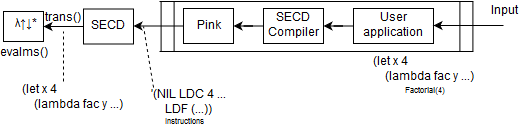
\includegraphics[scale=0.75]{secd_arch.png}
	\caption{``Effectively functional'' \mslangStar with SECD tower above it}\label{secd_tower_arch}
\end{figure}

\section{Contributions}
\begin{itemize}
	\item Generalized framework for collapsable towers. A generilzation of \cite{amin2017collapsing} for ``heterogeneous'' towers
	\item Extension of the core \mslang to support side effects, combining previous insights into multi-level $\lambda$ \cite{nielson1996multi} and work on side-effects in partial evaluators \cite{asai1997partial}.
	\item Denotational account of original base language/Pink and the new \mslang (including a store, which was not part of \cite{danvy1988intensions})
	\item Development a CESK-style abstract machine/ abstract interpreter for said extended \mslang
	\item Form a basis for further work on towers by providing a stage polymorphic base evaluator capable of modelling functional or imperative languages
	\item Mimick a practical tower through a SECD machine on top of the base evaluator and show compilation without staging commands throughout the tower
	\item Theoretical proposal of how one might achieve collapsing in practice
\end{itemize}

We deviate from traditional research in reflective towers in that we do not develop a separate language that demonstrates reflective tower capabilities and part from the constraints of metacircularity and reflection.
Instead of generating levels in the tower dynamically through reflection and reification operators we construct a pre-determined tower resembling towers of interpreters in practice. We demonstrate initially how meta-circularity and reflection
eases the collapsing process and then wire the tower in a way that breaks key implicit assumptions of said technique. Finally we propose a generalization of the original framework that deals with the constraints such a semantic gaps and lack of
reflection and reification. We evaluate the framework on a set of abstract machines that are convenient to implement in Lisp-like fashion but are capable of modelling a broad set of functional and non-functional language properties.

\section{Normalization By Evaluation (NBE)}
Useful \href{http://cs.ioc.ee/ewscs/2009/dybjer/mainPalmse-revised.pdf}{Slides}
\href{http://www.cse.chalmers.se/~abela/univnbe.pdf}{NBE paper}
\href{http://homepages.inf.ed.ac.uk/slindley/nbe/nbe-cambridge2016.pdf}{More slides}
\href{https://www.microsoft.com/en-us/research/wp-content/uploads/2016/07/supercomp-by-eval.pdf?from=http%3A%2F%2Fresearch.microsoft.com%2Fen-us%2Fum%2Fpeople%2Fsimonpj%2Fpapers%2Fsupercompilation%2Fsupercomp-by-eval.pdf}{Supercompilation by Evaluation}
\href{http://citeseerx.ist.psu.edu/viewdoc/download?doi=10.1.1.630.2123&rep=rep1&type=pdf}{Supercompilation and Normalization by Evaluation}

\section{Type-Directed Partial Evluation (TDPE)}
\cite{grobauer2001second}

\subsection{Staging}
There are two types of partial evaluation methodologies \cite{jones1993partial}:
\begin{itemize}
	\item Offline partial evaluation
	\item Online partial evaluation \cite{cook2011tutorial}
\end{itemize}
Namin et al. \cite{amin2017collapsing}, propose two languages Pink and Purple. Pink uses a form of online partial evaluation but requires manual staging facilities. Purple relies on LMS for automatic binding time analysis and staging
which limits it to offline partial evaluation and thus relies on further optimization heuristics to achieve the same level of program specialization in the generated code as Pink.

Our language extends Pink with side effects and a stack machine that makes use of pointer like semantics for Lisp-like cons pairs. Thus we build on top of the NBE-style lift operator for staging. However, calling into
the base-level lift requires knowledge about its use to be passed from the layers above. We can employ several strategies of doing this:
\begin{itemize}
	\item A basic approach exposes the base layer staging operation to the level above. This is how the original Pink implementation works.
	\item At every layer \textit{deduce} whether we need to call the underlying interpreter staging operator
	\begin{itemize}
		\item This requires every level to include an implementation of such staging operations
	\end{itemize}
	\item A mixture of passing staging operations to the layer below or implementing ones own operators
	\item Find a method of passing staging decisions through each layer in a generic way without intrusive changes to the evaluators of the layers
	\item Decide about calling staging operations at a particular point in the tower and apply previous points
\end{itemize}
We are interested in the last two point. In heterogeneous and practical towers a programmer does not have the liberty to introduce intrusive changes along each layer.
The original Pink implementation assumes we are allowed to make arbitrary changes to evaluators. It effectively adds tags to the emitted representation of a layer above and lets the layer below infer from these tags
what tag it itself should pass to the next layer, eventually calling the base-level Lift term.

\section{Why do we want to collapse towers? (aren't they pretty?)}
The main reason is performance. The key realization of partial evaluation that lead to its development is that interpreters do redundant work but we can make it so they don't. Program specialization
is simple and attractive on paper but poses significant engineering challenges and has not seen widespread adoption (until recent increasingly successful work on interpreter virtualization \cite{wurthinger2013one}).

Binding time analysis is one of the obstacles of program specialization. The program specializer needs to decide, either automatically or with assistance from the programmer, which data to treat as static and which as dynamic. Simple divisions
can lead to code explosion or inefficient code generation, or worse, to non-termination of the specializer. This problem is known as \textit{division} and is one of the key differences between offline and online PE techniques \cite{jones1993partial}.

An curious use-case for staging towers of interpreters started with the challenge of compiling the reflective language proposed by Asai et al. \cite{asai1997partial, asai2015compiling}. The authors are able to compile a Lisp-like reflective language, built through
the infinite tower of interpreters model \cite{smith1982reflection,wand1988mystery,danvy1988intensions}, with respect to the initial semantics of the tower. Amin et al. \cite{amin2017collapsing} then extended this work to allow compilation of such towers
under modified semantics i.e. dynamically changing behaviour of individual interpreters. An interesting consequence demonstrated in their paper is the ability to derive translators in the process of collapsing.

\subsubsection{Example of Deriving Translators}
A trivial but useful example is logging. Given the tower in figure \ref{logging_translator_tower} we want to keep the added \textit{useful} behaviour of $I_3$ while removing the \textit{unuseful} other work of interpreting an intermediate representation. The interpretation
of the IR of the level above is a mere accidental consequence of design instead of a necessity. We claim this work to be \textit{interpretative overhead} and defer its quantification by benchmarks to a later section.

Collapsing the tower achieves exactly what we wanted, base-language (here the compilation target language) expressions including logging specialized to the user-level program.

A restriction with this method is its reliance on meta-circularity and reflection and other unsafe techniques:
\begin{itemize}
	\item we are able ``inject'' the logging evaluator into tower because of its meta-circularity
	\item we expose staging operators throughout the tower through simple string manipulation
	\item instrumentation relies on meta-circularity since we simply redefine how constructs are evaluated before injecting the evaluator
	\item modification of semantics of the tower are done via reflection (ELABORATE)
\end{itemize}

Nonetheless, it is an interesting consequence of compiling towers that we can collect side-effects in individual levels (in the original framework at no extra cost), and have an interpreter
above exhibit them. Analogous to a sieve, we take a coarse-grained collection of functionality, loosen it and extract only the individual grains we want. Imagine the sieve being coated with a thin film. All grains passing through
will now have the film applied to them. Here sieves are the levels below and grains are the levels above. (REFINE ANALOGY)

Our study examines this property by testing the limits of how we can get the side effects to stick to interpreters in a useful way. One could imagine optimizations, parallelization or instrumentation as possible use cases. Under certain side-effects, we may, however,
reach limits in terms of security (TROJANS IN HYPERVISORS) or ability to reason about a system. We are interested in the extent of these limits. (concurrency as a side-effect: instead of launching missiles we launch threads)

\section{Towers in the Wild}
To provide a real-world analogy of the language towers we are constructing describe some existing arrangements of multi-interpreter systems below:
\begin{itemize}
	\item \href{https://github.com/jashkenas/coffeescript/wiki/List-of-languages-that-compile-to-JS}{Here} is a list of languages that are built on top of JavaScript. This is a three-level interpreter system: User-application<->DSL<->JavaScript Interpreter
	\item \href{https://github.com/vindarel/languages-that-compile-to-python#other-languages-that-target-the-python-platform}{Here} is a list of languages that compile to Python.
	\item \href{https://github.com/copy/v86}{v86} is a x86 CPU emulator written in JavaScript. This closely resembles our stack machine that is evaluated in both Pink or the Base language's multi-stage evaluator
	\item \href{http://6502asm.com/}{6502asm} is a microcontroller emulator in JavaScript
\end{itemize}

\section{On Side-effects and Dynamic Semantics of Programming Languages}
References:
\begin{itemize}
	\item 
\end{itemize}

\subsection{Adding Levels}
Added stack machine
DIAGRAMS

\subsection{Result of collapsing}

\subsection{Cost of Emulation (or interpreteation)}
% https://www.quora.com/Why-are-emulators-so-badly-optimized
% https://stackoverflow.com/questions/448673/how-do-emulators-work-and-how-are-they-written
\cite{steil2004dynamic}
\href{http://materials.dagstuhl.de/files/17/17061/17061.PaulH.J.Kelly.Slides.pdf}{Turing Tax}
\href{https://www.doc.ic.ac.uk/~phjk/AdvancedCompArchitecture/Lectures/pdfs/Ch01-TuringTaxDiscussionV02.pdf}{Turing Tax specific slides}

\section{Methodologies}
\subsection{Abstract Machines}


\bibliographystyle{IEEEtran}
\bibliography{lit_review}

\end{document}